\documentclass[aspectratio=169,11pt]{beamer}
\usepackage[T1]{fontenc}
\usepackage{lmodern,amsmath,amssymb,mathtools,bm,booktabs,array,graphicx,tikz}
\usetikzlibrary{arrows.meta,positioning,calc,decorations.pathreplacing,patterns}
\definecolor{ink}{HTML}{17344D}\definecolor{accent}{HTML}{087E8B}\definecolor{pale}{HTML}{EDF5F5}\definecolor{gold}{HTML}{AD6B19}
\providecommand{\dd}{\,\mathrm{d}}\providecommand{\R}{\mathbb{R}}
\providecommand{\E}{\mathbb{E}}\providecommand{\Var}{\operatorname{Var}}
\providecommand{\Cov}{\operatorname{Cov}}\providecommand{\diag}{\operatorname{diag}}
\providecommand{\norm}[1]{\left\lVert#1\right\rVert}
\providecommand{\abs}[1]{\left|#1\right|}
\usefonttheme{professionalfonts}
\setbeamercolor{normal text}{fg=black,bg=white}
\setbeamercolor{frametitle}{fg=ink,bg=white}
\setbeamercolor{title}{fg=ink}\setbeamercolor{structure}{fg=accent}
\setbeamercolor{block title}{fg=ink,bg=pale}\setbeamercolor{block body}{fg=black,bg=pale!40}
\setbeamercolor{alerted text}{fg=accent}
\setbeamerfont{frametitle}{size=\Large,series=\bfseries}
\setbeamerfont{title}{size=\LARGE,series=\bfseries}
\setbeamertemplate{navigation symbols}{}
\setbeamersize{text margin left=.7cm,text margin right=.7cm}
\setbeamertemplate{frametitle}{\vspace{.18cm}\insertframetitle\par\vspace{.1cm}{\color{accent}\hrule height .6pt}\vspace{.12cm}}
\newcommand{\notestarget}{notes.pdf}\newcommand{\noteslabel}{Notes}
\setbeamertemplate{footline}{\hspace{.7cm}\color{ink}\scriptsize Computational Cardiology\quad\href{\notestarget}{\noteslabel}\hfill\insertframenumber\,/\,\inserttotalframenumber\hspace{.7cm}\vspace{.18cm}}
\setbeamercovered{invisible}
\hypersetup{pdfauthor={Zan Ahmad},pdftitle={Probability calibration and missing-modality evaluation},pdfpagemode=UseNone}
\begin{document}
\begin{frame}[plain]\vfill
{\small\color{accent} Computational Cardiology \quad Lecture 16}\par\medskip
{\raggedright\hyphenpenalty=10000\exhyphenpenalty=10000\LARGE\bfseries\color{ink} Probability calibration and missing-modality evaluation}\par\bigskip
Zan Ahmad\par\smallskip
{\small Fall 2024}\par\vfill\end{frame}
\renewcommand{\notestarget}{notes.pdf\#note-group-level-scores-and-prediction-tasks}
\begin{frame}[t,fragile,label=slide-three-properties-of-a-score]{Three properties of a score}
Ranking concerns ordering, classification concerns a threshold, and probability prediction concerns numerical event probabilities.\pause{} Improving one need not improve all three.
\end{frame}
\renewcommand{\notestarget}{notes.pdf\#note-group-level-scores-and-prediction-tasks}
\begin{frame}[t,fragile,label=slide-aggregate-repeated-observations]{Aggregate repeated observations}
\[p_g=\sigma((z_{g1}+z_{g2})/2).\]\pause{} This is generally different from averaging the two probabilities.
\end{frame}
\renewcommand{\notestarget}{notes.pdf\#note-a-paired-missing-modality-intervention}
\begin{frame}[t,fragile,label=slide-the-paired-modality-comparison]{The paired modality comparison}
A-only and AB predictors are evaluated on the same unseen groups.\pause{} Changing the eligible cohort would confound the effect of adding B.
\end{frame}
\renewcommand{\notestarget}{notes.pdf\#note-imputation-missingness-indicators-and-a-fixed-cohort}
\begin{frame}[t,fragile,label=slide-represent-a-missing-measurement]{Represent a missing measurement}
\[B^*=\begin{cases}B,&\text{observed},\\m_B^{train},&\text{missing},\end{cases}\qquad r_B=\boldsymbol1_{\{B\ \text{missing}\}}.\]\pause{} The indicator distinguishes imputation from an observed median value.
\end{frame}
\renewcommand{\notestarget}{notes.pdf\#note-imputation-missingness-indicators-and-a-fixed-cohort}
\begin{frame}[t,fragile,label=slide-freeze-preprocessing]{Freeze preprocessing}
The training median, means and scales are reused for validation and testing.\pause{} The missingness indicator records absence; it does not recover the missing information.
\end{frame}
\renewcommand{\notestarget}{notes.pdf\#note-positive-temperature-scaling}
\begin{frame}[t,fragile,label=slide-temperature-scaled-probabilities]{Temperature-scaled probabilities}
\[p_T=\sigma(z/T),\qquad T>0.\]\pause{} The supplied experiment first sharpens logits by a declared factor $2.5$.
\end{frame}
\renewcommand{\notestarget}{notes.pdf\#note-positive-temperature-scaling}
\begin{frame}[t,fragile,label=slide-ranking-is-preserved]{Ranking is preserved}
\[z_i>z_j\quad\Longrightarrow\quad\sigma(z_i/T)>\sigma(z_j/T).\]\pause{} Positive temperature preserves ranking and ties, hence the pairwise AUC.
\end{frame}
\renewcommand{\notestarget}{notes.pdf\#note-positive-temperature-scaling}
\begin{frame}[t,fragile,label=slide-the-one-half-decision-is-preserved]{The one-half decision is preserved}
\[\sigma(z/T)\ge\tfrac12\quad\Longleftrightarrow\quad z\ge0.\]\pause{} Other fixed probability thresholds need not preserve their classifications.
\end{frame}
\renewcommand{\notestarget}{notes.pdf\#note-positive-temperature-scaling}
\begin{frame}[t,fragile,label=slide-fit-temperature-using-validation-likelihood]{Fit temperature using validation likelihood}
\[\widehat T=\arg\min_{T>0}\frac1N\sum_i[\log(1+e^{z_i/T})-y_i z_i/T].\]\pause{} The base model and all preprocessing remain fixed.
\end{frame}
\renewcommand{\notestarget}{notes.pdf\#note-proper-probability-scores-and-reliability-bins}
\begin{frame}[label=slide-the-brier-score-panel-1]{Sharpened AB scores}
\centering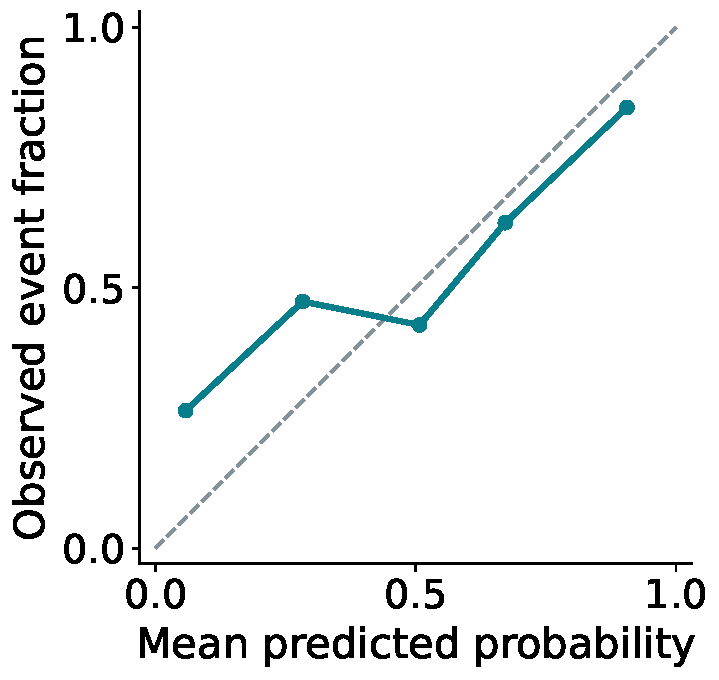
\includegraphics[width=.98\linewidth,height=.69\textheight,keepaspectratio]{presentation-figures/calibration-panel-1.pdf}\end{frame}
\renewcommand{\notestarget}{notes.pdf\#note-proper-probability-scores-and-reliability-bins}
\begin{frame}[label=slide-the-brier-score-panel-2]{Validation-calibrated AB}
\centering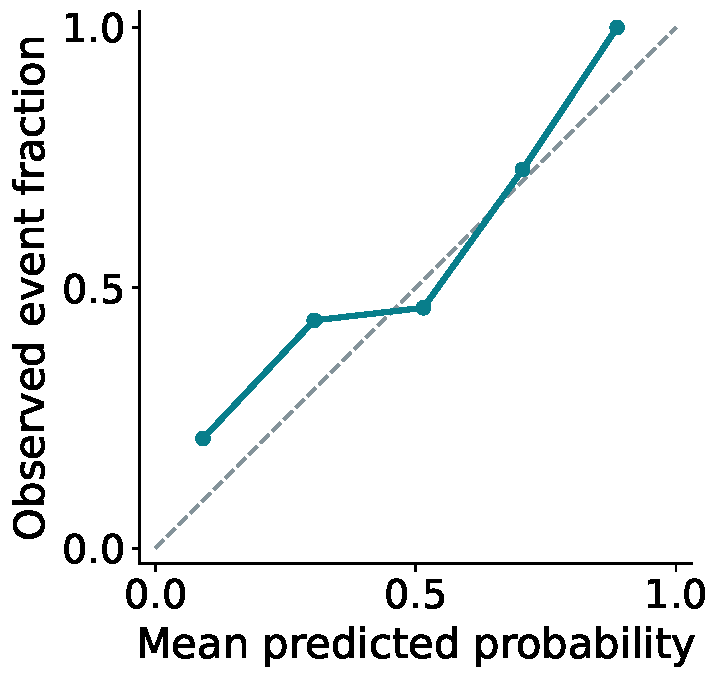
\includegraphics[width=.98\linewidth,height=.69\textheight,keepaspectratio]{presentation-figures/calibration-panel-2.pdf}\end{frame}
\renewcommand{\notestarget}{notes.pdf\#note-proper-probability-scores-and-reliability-bins}
\begin{frame}[t,fragile,label=slide-the-brier-score]{The Brier score}
\[\mathrm{Brier}=\frac1N\sum_i(p_i-y_i)^2.\]\pause{} It evaluates probabilities, not only the chosen classification threshold.
\end{frame}
\renewcommand{\notestarget}{notes.pdf\#note-proper-probability-scores-and-reliability-bins}
\begin{frame}[t,fragile,label=slide-conditional-probability-decomposition]{Conditional probability decomposition}
\[\mathbb E[(p-Y)^2\mid X]=(p-\eta)^2+\eta(1-\eta).\]\pause{} The minimum occurs at the true conditional event probability $\eta$.
\end{frame}
\renewcommand{\notestarget}{notes.pdf\#note-proper-probability-scores-and-reliability-bins}
\begin{frame}[t,fragile,label=slide-reliability-bins]{Reliability bins}
Each bin compares its mean forecast with its observed event fraction.\pause{} Counts determine how much information each point contains; an empty bin has no empirical fraction.
\end{frame}
\renewcommand{\notestarget}{notes.pdf\#note-a-paired-missing-modality-intervention}
\begin{frame}[label=slide-remove-b-while-retaining-the-same-groups-figure]{Brier score (lower is better)}
\centering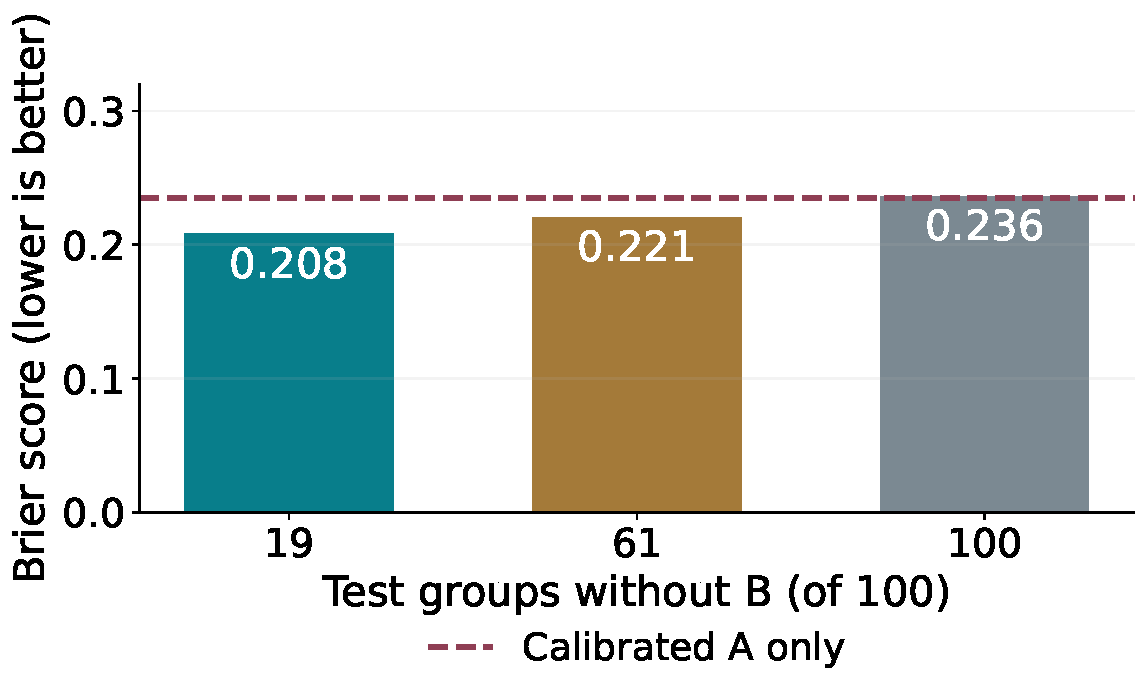
\includegraphics[width=.98\linewidth,height=.69\textheight,keepaspectratio]{presentation-figures/missing-modality-panel-1.pdf}\end{frame}
\renewcommand{\notestarget}{notes.pdf\#note-a-paired-missing-modality-intervention}
\begin{frame}[t,fragile,label=slide-remove-b-while-retaining-the-same-groups]{Remove B while retaining the same groups}
Replace B by the frozen missing-data rule and retain every test outcome.\pause{} The change measures sensitivity to this particular information-loss intervention.
\end{frame}
\renewcommand{\notestarget}{notes.pdf\#note-proper-probability-scores-and-reliability-bins}
\begin{frame}[t,fragile,label=slide-auc-and-probability-quality-can-separate]{AUC and probability quality can separate}
Positive temperature leaves AUC unchanged while changing Brier score and likelihood.\pause{} A better probability score on one sample is an empirical result, not an algebraic guarantee.
\end{frame}
\renewcommand{\notestarget}{notes.pdf\#note-calibration-and-distribution-dependence}
\begin{frame}[t,fragile,label=slide-distribution-dependent-calibration]{Distribution-dependent calibration}
\[P_{future}(Y=1\mid z)\ne P_{validation}(Y=1\mid z)\]\pause{} can invalidate a fitted calibration map even when the implementation is unchanged.
\end{frame}
\end{document}
